HPO permite extraer los genes anotados a un fenotipo, por lo que estos han sido descargados y utilizando la API de StringDB se han obtenido la red de interacción (\textit{Figura} \ref{fig:network}).
Se ha establecido el umbral de \textit{combine\_score} a 700.

\begin{figure}[h]
	\centering
	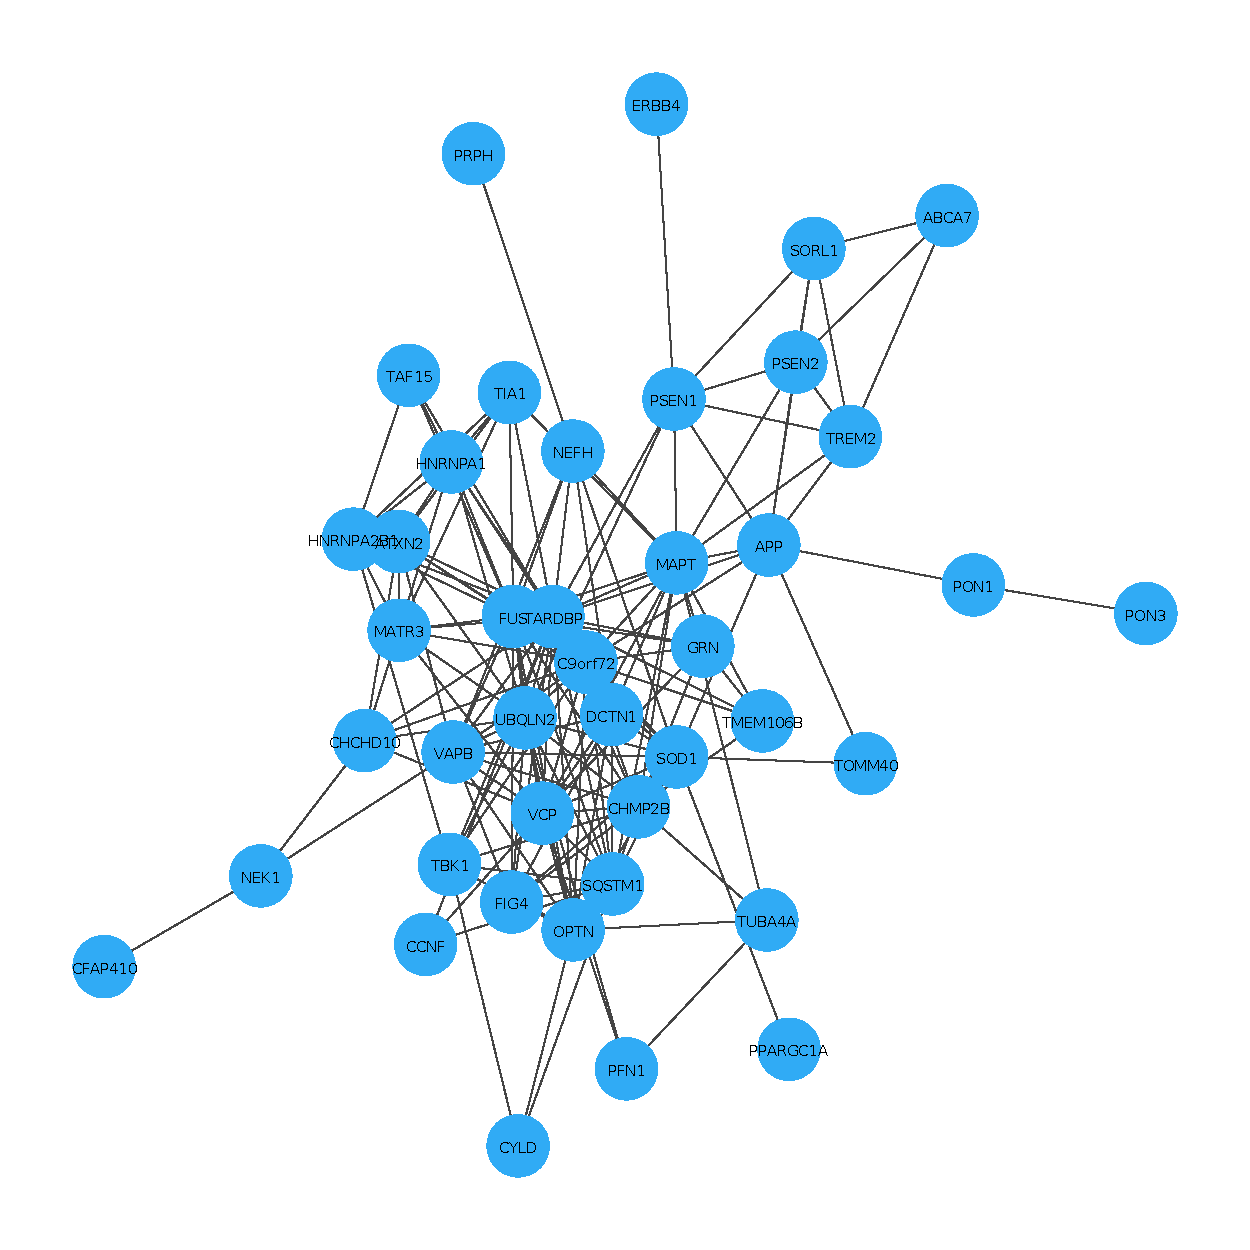
\includegraphics[width=0.90\linewidth]{../results/plots/network/network.pdf}
	\caption{Red de interacción proteína-proteína de los genes del HPO (HP:0002145) obtenida mediante la API de StringDB con un filtro de 400 del combine score}
	\label{fig:network}
\end{figure}

En la \textit{Figura \ref{fig:network}} observamos que proteínas con un número de conexiones respecto a otras. 
Un análisis en mayor profundidad de la red se presenta en la \textit{Tabla \ref{tab:NetworkMetrics}}.


\begin{table}[h!]
	\centering
	\caption{Resumen de Métricas de la Red PPI}
	\label{tab:NetworkMetrics}
	\begin{tabular}{ll}
		\toprule
		\textbf{Categoría} & \textbf{Métrica y Valor} \\
		\midrule
		\multirow{2}{*}{\textbf{Tamaño de la Red}} 
		& Número de nodos: 42 \\
		& Número de aristas: 171 \\
		\midrule
		\multirow{2}{*}{\textbf{Grado}} 
		& Grado promedio: 8.14 \\
		& Desviación estándar del grado: 5.93 \\
		\midrule
		\multirow{3}{*}{\textbf{Conectividad}} 
		& Grafo conectado: Sí \\
		& Conectividad de nodos: 1 \\
		& Conectividad de aristas: 1 \\
		\midrule
		\multirow{2}{*}{\textbf{Densidad y Sparsity}} 
		& Densidad: 0.199 \\
		& Esparcidad: 0.801 \\
		\midrule
		\multirow{2}{*}{\textbf{Cercanía (Closeness)}} 
		& Cercanía promedio: 0.456 \\
		& Desviación estándar de cercanía: 0.093 \\
		\midrule
		\multirow{2}{*}{\textbf{Centralidad (Betweenness)}} 
		& Betweenness promedio: 26.50 \\
		& Desviación estándar de betweenness: 39.56 \\
		\midrule
		\multirow{3}{*}{\textbf{Transitividad}} 
		& Transitividad local promedio: 0.550 \\
		& Desviación estándar de transitividad local: 0.322 \\
		& Transitividad global: 0.520 \\
		\midrule
		\multirow{3}{*}{\textbf{Otras Propiedades}} 
		& Asortatividad: -0.018 \\
		& Diámetro: 6 \\
		& Longitud de camino promedio: 2.293 \\
		\bottomrule
	\end{tabular}
\end{table}

En HPO se tenían 52 genes relacionados con nuestro fenotipo, pero en la red filtrado tan solo hay 42 proteínas. 
Por tanto hay diez genes, que no interaccionan con las otras proteínas de la red con un alto umbral de confianza. 
Con un umbral inferior al establecido,  estos genes estarían en la red, pero la significancia biología de las interacciones no sería fiable.

El grado medio de los nodos, correspondiente al número de conexiones de un nodo, es 8.14, un valor considerablemente alto si tenemos en cuenta el número de nodos presentes en la red. En total, la red tiene 171 conexiones ente proteínas.
Hay un valor significativo de desviación típica del grado de los nodos. Un mejor análisis de las distribución de los grados se presenta en la \textit{Figura \ref{fig:degree}}. 
En esta figura, observamos que la gran mayoría de las proteínas, tienen grados relativamente bajos, inferiores a la medio. Encontramos un par de proteínas, con grados superiores a 20, lo que indica que están conectados a más de la mitad de las proteínas de la red.
Estos nodos altamente conectados podrían ser hubs (FUS, TARDBP). %cre que no lo son (mirar conectividad y centralidad) %aunque si los quitas el grafo sigue conexo, mirar en que pathways están incluidos
Si nos fijamos en la densidad del grafo, vemos que tenemos una red con baja densidad, hay pocas conexiones con respecto a las posibles.


\begin{figure}[h]
	\centering
	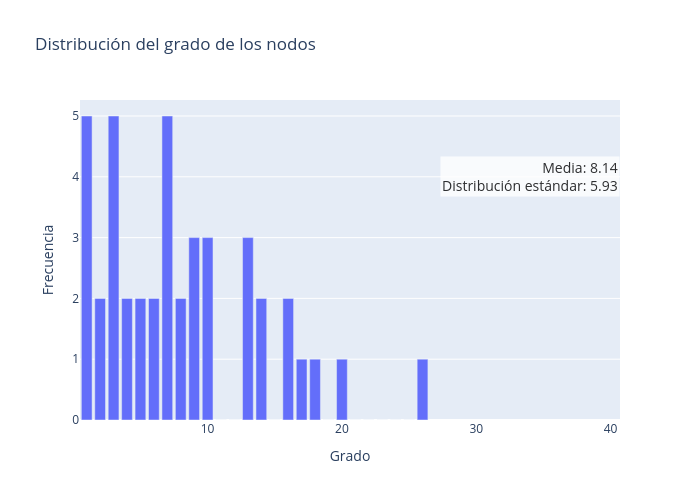
\includegraphics[width=1\linewidth]{../results/plots/network/degree_distribution.png}
	\caption{Distribución de los grados de los nodos, mediante un histograma, de la red de interacción.}
	\label{fig:degree}
\end{figure}

La red obtenida es un grafo conexo (ver \textit{Figura \ref{fig:network}}), el análisis de la conectivadad llevado a cabo muestra que existe una conectividad tanto de vértice (nodo) como de arista de 1.
Esto indica que exiten uno o varios nodos/aristas que si son eliminados desconectan el grafo. Se ha determinado que estos nodos son las proteínas NEK1, SOD1, APP, PON1, NEFH Y PSEN1.

Las siguientes métrica analizadas son la centraliad y cercanía, en la \textit{Tabla \ref{tab:NetworkMetrics}} se muestra la media y desviación, 
ya que se tratan de métricas que se miden por cada nodo. Para ambas métricas destaca una de las dos proteínas antes mencionadas con el grado,TARDBP.
%añadir más explicación

\begin{figure}[h]
	\centering
	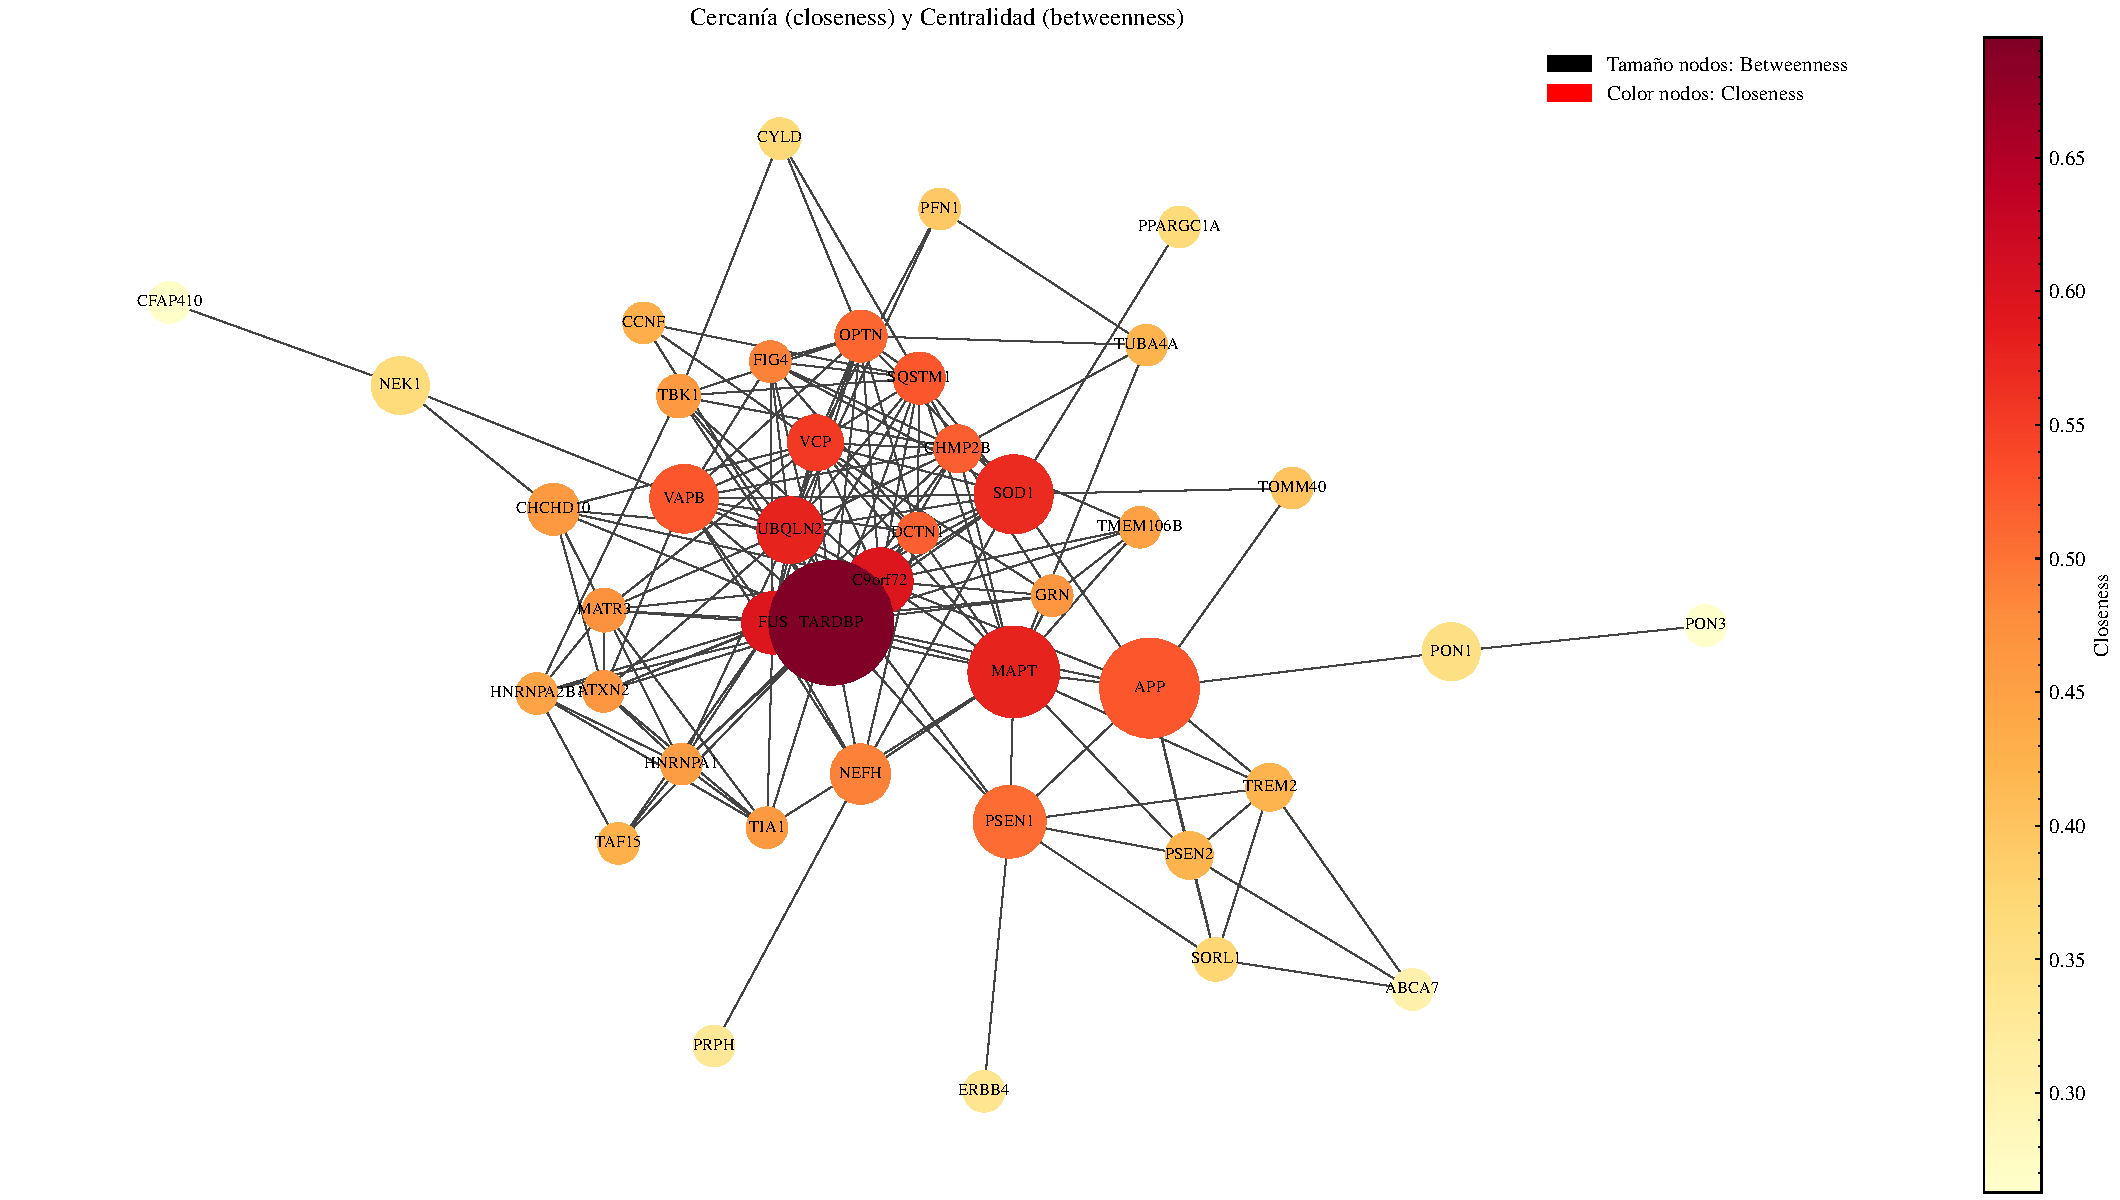
\includegraphics[width=0.98\linewidth]{../results/plots/network/closeness_betwennes_graph.pdf}
	\caption{Representación visual de la relación entre closeness (cercanía) y betweenness (centralidad de intermediación) para los nodos de la red. 
    El tamaño de los nodos ha sido establecido en base al valor de centralidad obtenido y el valor de cercanía se establece con el color del nodo.}
	\label{fig:closeness_betweenness}
\end{figure}

Finalmente podemos mencionar la transitividad, probabilidad de que los vecinos de un nodo estén también conectados entre sí.
Tanto la transitividad local como la global tienen valores parecidos, entorno a 0.5. Puntualizar que para el calculo de la transitividad local, se han obviado aquellos nodos que dan valores de NaN debido a que solo presentan un vecino.
